\documentclass[spanish,xcolor=table]{beamer}
\usepackage[spanish]{babel}
\selectlanguage{spanish}
\usepackage[utf8]{inputenc}
\mode<presentation> {

%----------------Beamer Themes--------------------

\usetheme{Boadilla}

%--------------------Beamer Font & Colors----------

\usecolortheme{seahorse}

%-------------------Beamer Options --------------------

\setbeamertemplate{navigation symbols}{} % To add the navigation symbols from the bottom of all slides comment this line
}

%-------------------Package----------------------------
\RequirePackage{natbib}
\usepackage{graphicx} 
\usepackage{booktabs} % use of \toprule, \midrule and \bottomrule in tables
\usepackage{tikz}
\usepackage{pgfplots}
\usepackage{multirow}
\usepackage{multicol}
\usepackage{amsmath}
\usepackage{hhline}
\usepackage[export]{adjustbox} %para posicionar imagenes(ej, left, right)

%---Librerias de Tikz -----------------------------
\usetikzlibrary{arrows,calc}
\usetikzlibrary{intersections}
\usetikzlibrary{pgfplots.fillbetween}
\usetikzlibrary{patterns}
\usetikzlibrary{plotmarks}
\usetikzlibrary{calc}
\usetikzlibrary{matrix}
\usetikzlibrary{positioning}
\usepackage{relsize}
\usepackage[nointegrals]{wasysym}
\usepackage{caption}
\usepackage{bigints}
\usepackage{xcolor}
%---------------------------------------------------------------------------------

%-----------Tikz Layers---------------------------------
\pgfdeclarelayer{ft}
\pgfdeclarelayer{bg}
\pgfsetlayers{bg,main,ft}
%---------------------------------------------------------

%--------Definiciones de Operadores --------------
\DeclareMathOperator*{\argmax}{arg\,max}
\def\checkmarkt{\tikz\fill[scale=0.4](0,.35) -- (.25,0) -- (1,.7) -- (.25,.15) -- cycle;} 
\newcommand{\bigqm}[1][1]{\text{\larger[#1]{\textbf{?}}}}
\let\Tiny=\tiny % fix issue font name beamer
\makeatletter

\newcommand\mathcircled[1]{%
  \mathpalette\@mathcircled{#1}%
}
\newcommand\@mathcircled[2]{%
  \tikz[baseline=(math.base)] \node[draw,circle,inner sep=1pt] (math) {$\m@th#1#2$};%
}

%north west lines pattern density ajusted
\pgfdeclarepatternformonly[\LineSpace,\LineSpaceColor]{MNWL}{\pgfqpoint{-1pt}{-1pt}}{\pgfqpoint{\LineSpace}{\LineSpace}}{\pgfqpoint{\LineSpace}{\LineSpace}}%
{
    \pgfsetcolor{\tikz@pattern@color}
    \pgfsetlinewidth{0.4pt}
    \pgfpathmoveto{\pgfqpoint{0pt}{\LineSpace}}
    \pgfpathlineto{\pgfqpoint{\LineSpace + 0.1pt}{-0.1pt}}
    \pgfsetstrokecolor{\LineSpaceColor}%        % <-- added
    \pgfusepath{stroke}
}
\makeatother

\newdimen\LineSpace
\tikzset{
    line space/.code={\LineSpace=#1},
    line space=6pt, %this ajust density of MNWL
    line color/.store in=\LineSpaceColor,      % <-- added
    line color=black,
} %line set color in custom parttern check line 665-667 for an example

%----------------------------------------------------------------------------------------
%	           Slide Inicial
%----------------------------------------------------------------------------------------
 
\title[ECO -TS101]{Econometr\'\i{}a de Series de Tiempo} 
\subtitle{T\'opico IV.- Cointegration Analysis}

%Profesores

\author{Marcelo Villena Ch., PhD} 

%-----------------------------------------------------------------

\institute[UAI] % Your institution as it will appear on the bottom of every slide, may be shorthand to save space
{
Universidad Adolfo Ib\'a\~nez 
 \\ % institution for the title page
\medskip
}
\date{} % Date, can be changed to a custom date

%-------------------Figure Settings-------------------
\pgfplotsset{ % Here we specify options for all figures in the document
  compat=1.8, % Which version of pgfplots do we want to use?
  legend style = {font=\small\sffamily}, % Legends in a sans-serif font
  label style = {font=\small\sffamily} % Labels in a sans-serif font
}

%-----Color definitions-------------
\colorlet{ColorG}{black!60!green}
\colorlet{ColorR}{black!60!red}
\colorlet{ColorB}{black!60!blue}
\colorlet{ColorY}{black!40!yellow}
%-----------------------------------

\begin{document}

\begin{frame}

\begin{figure}[t!]

\includegraphics[scale=0.1]{Logo.jpg}
\end{figure}
\titlepage % Print the title page as the first slide
\end{frame}

\begin{frame}
\frametitle{Contenidos} 
\tableofcontents % Lista de contenidos, carga la instruccion \section{} y \subsection{} 
\end{frame}


%----------------------------------------------------------------------------------------
%	PRESENTATION SLIDES
%----------------------------------------------------------------------------------------

%------------Slides------------------------------------
%---------------------Slide 3--------------------------
\begin{section}{Introducci\'on}
\begin{frame}
\frametitle{Cointegraci\'on}
\textbf{Introducci\'on}

Si dos o más series temporales no estacionarias siguen un camino común (o  de equilibrio) a largo plazo, podemos hablar de cointegraci\'on. La prueba cli\'asica de cointegraci\'on se reduce a determinar si una combinaci\'on lineal de la serie es estacionaria o no. Si, por ejemplo, dos series temporales est\'an cointegradas por un factor com\'un (vector de cointegraci\'on), no es posible utilizar un enfoque VAR est\'andar. Tenemos que dar cuenta de esta relaci\'on y utilizar un modelo de correcci\'on de errores para obtener resultados correctos.

\end{frame}
\end{section}


%---------------------------------------------------------
%---------------------Slide 4--------------------------
\begin{section}{Cointegraci\'on}
\begin{frame}
\frametitle{Cointegraci\'on}

Suponga que $Y_t = I(1)$ y $X_t=I(1)$. Entonces $Y_t$ y $X_t$ est\'an cointegradas, $CI(1,1)$, si existe un $\beta$, tal que $Y_t - \beta X_t = \epsilon_t = I(0)$. Esto implica que hay una relaci\'on de largo plazo entre $Y_t$ y $X_t$,  es decir ellas no se ``separan” a trav\'es del tiempo. De aqu\'\i{} la relaci\'on, $Yt= \beta X_t + \epsilon_t$, tiene sentido.\\
\vspace{4mm}	
Si $Y_t$ y $X_t$ no est\'an cointegradas, es decir, $\epsilon_t$ tambi\'en es $I(1)$, entonces, $Y_t$ y $X_t$ se separar\'an cada vez más a trav\'es del tiempo, y por lo tanto no existir\'a una relaci\'on de largo plazo entre dichas variables. Cualquier regresi\'on de $Y_t$ sobre $X_t$ es ``Espuria”.


\end{frame}

%---------------------------------------------------------
%---------------------Slide 5--------------------------
\begin{frame}
\frametitle{Cointegraci\'on}

En general, si $Y_t$ y $X_t$ son ambas $I(d)$, entonces $Y_t$ y $X_t$ son $CI(d,b)$ si $Yt - \beta X_t = \epsilon_t  = I(d-b), b>0.$\\
 \vspace{4mm}	
Si si $Y_t$ y $X_t$ est\'an cointegradas, esto significa que es posible modelar la relaci\'on de largo plazo entre $Y_t$ y $X_t$. Esta es una estrategia de modelamiento alternativa a eliminar la tendencia a trav\'es de diferenciaci\'on. El procedimiento de eliminar la tendencia en general, pierde informaci\'on. \\
\vspace{4mm}	
Por lo tanto, es posible aplicar un procedimiento de ``Cointegraci\'on de temporada" m\'as que tratar de eliminar el efecto de temporada diferenciando.\\

\end{frame}
\end{section}

%---------------------------------------------------------
%---------------------Slide 6--------------------------
\begin{section}{Test de Cointegraci\'on de Engle-Granger}
\begin{frame}
\frametitle{Test de Cointegraci\'on de Engle-Granger, ver \cite{engle1987co}}

Estimar le regresi\'on cointegrada, $Y_t = \beta X_t + \epsilon_t = I(0)$ usando MCO para obtener los residuos $e_t$. Aplicar el test de Dickey-Fuller (DF) y/o el test de Dickey-Fuller Aumentado (ADF) para examinar si los residuos tienen ra\'{i}ces unitarias. \\

\vspace{4mm}	

Si la hip\'otesis de ra\'{i}ces unitarias no es rechazada, esto implica que $\epsilon_t$ es $I(1)$, lo cual implica que $Y_t$ y $X_t$ NO est\'an cointegradas. Es importante notar que los valores cr\'{i}ticos para los test DF y ADF no son validos para ser usados para Cointegraci\'on. Engle y Granger han calculado los valores cr\'{i}ticos apropiados.

\end{frame}
\end{section}

%---------------------------------------------------------
%---------------------Slide 7--------------------------
\begin{section}{Modelo de Correcci\'on de Errores}
\begin{frame}
\frametitle{Modelo de Correcci\'on de Errores}

Si $Y_t$ y $X_t$ est\'an cointegradas, entonces hay una relaci\'on de largo plazo entre estas series y la din\'amica de corto plazo de esta relaci\'on puede ser descrita por el modelo de correcci\'on de errores (ECM).\\

\vspace{4mm}	
Relación de largo plazo:\\
 
\begin{equation}
Y_t = \beta X_t  + \epsilon_t 
\end{equation}

\end{frame}
%---------------------------------------------------------
%---------------------Slide 8--------------------------
\begin{frame}
\frametitle{El Modelo de Correcci\'on de Errores}

El modelo de correcci\'on de errores, es decir la din\'amica de corto plazo viene dada por:\\

\begin{equation}
\triangle Y_t = \alpha \triangle X_t + \phi [Y_{t-1} - \beta X_{t-1} ] + \epsilon_t 
\end{equation}

donde $\epsilon t$ = white noise, es decir $I(0)$.\\
 \vspace{4mm}	

Interpretaci\'on: el cambio actual en $Y_t$ consiste de dos componentes:\\

\only<1->{
\begin{itemize}
\item[(i)] $\alpha \triangle X_t$: la respuesta de corto plazo a los cambios actuales en $X_t$, y
\item[(ii)] $\phi [Y_{t-1} - \beta X_{t-1} ]$: la correcci\'on parcial de la desviaci\'on previa de $Y_t$ de su nivel deseado de largo plazo.
\end{itemize}
}

\end{frame}

%---------------------------------------------------------
%---------------------Slide 9--------------------------
\begin{frame}
\frametitle{Procedimiento de Estimaci\'on}

El procedimiento de dos pasos de Engle-Granger\\

\only<1->{
\begin{itemize}
\item[(i)] Estimar la regresi\'on de Cointegraci\'n para obtener una estimaci\'on del par\'ametro de largo plazo, y entonces,
\item[(ii)] Usar los residuos para estimar el modelo de correcci\'on de errores.
\end{itemize}
}

\end{frame}
%---------------------------------------------------------
%---------------------Slide 10--------------------------
\begin{frame}
\frametitle{Cointegration in practice}
\textbf{Ejemplo Modelo IPSA - CU - S$\&$P}

Analizaremos la relaci\'on de largo plazo entre la bolsa chilena, el IPSA, la bolsa americana, el $S\&P$ 500, y el precio del cobre, cu. En particular probaremos la hip\'otesis de contegraci\'on. Primero presentamos el test de estacionaridad para las tres variables.

\only<1|handout:1>{
\begin{exampleblock}{C\'odigo en R}

library(tseries) $\#$ df, adf\\
library(dynlm) $\#$ time series regression\\

mydata$<-$read.csv (``cointegration.csv")\\
ipsa$<-$ts(mydata$\$$IPSA,frequency=12, start = c(2010,1))\\
cu$<-$ts(mydata$\$$CU,frequency=12, start = c(2010,1))\\
sp$<-$ts(mydata$\$$s.p,frequency=12, start = c(2010,1))\\
summary(mydata)\\
\\
adf.test(diff(ipsa)); adf.test(diff(sp)); adf.test(diff(cu))\\

\end{exampleblock}
}

\end{frame}

%---------------------------------------------------------
%---------------------Slide 11--------------------------
\begin{frame}
\frametitle{Cointegration in practice}
\textbf{Ejemplo Modelo IPSA - CU - S$\&$P}

\begin{figure}[t!]
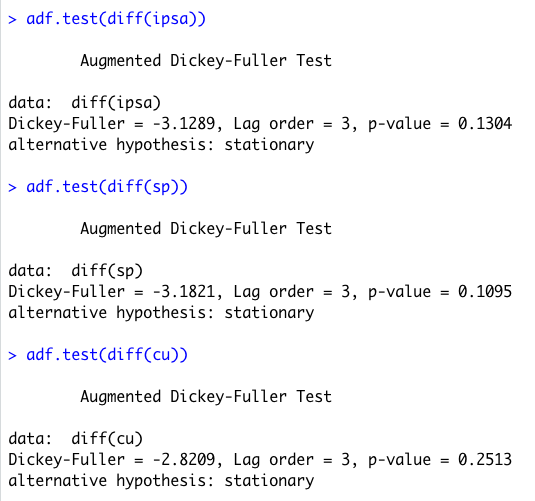
\includegraphics[scale=0.5]{adf.png}
\end{figure}

\end{frame}

%---------------------------------------------------------
%---------------------Slide 12--------------------------
\begin{frame}
\frametitle{Cointegration in practice}
\textbf{Ejemplo Modelo IPSA - CU - S$\&$P}

Ahora ejecutamos el modelo de cointegraci\'on de dos etapas Engle-Granger. Primero buscamos una relaci\'on de largo plazo de las variables, y encontramos que la relaci\'on IPSA y CU es la m\'as fuerte. \\
\\
\only<1|handout:1>{
\begin{exampleblock}{C\'odigo en R}

ipsa.reg1 $<-$ dynlm(ipsa $\string ~$ cu + sp)\\
summary(ipsa.reg1)\\
ipsa.reg2 $<-$ dynlm(ipsa $\string ~$ L(cu, 1:3))\\
summary(ipsa.reg2)\\
ipsa.reg3 $<-$ dynlm(ipsa $\string ~$ cu)\\
summary(ipsa.reg3)\\
residuos $<-$ ipsa.reg3[[``residuals"]]\\
plot(residuos); adf.test(residuos); qqnorm(residuos); qqline(residuos)\\
\end{exampleblock}
}

\end{frame}

%---------------------------------------------------------
%---------------------Slide 13--------------------------
\begin{frame}
\frametitle{Cointegration in practice}
\textbf{Ejemplo Modelo IPSA - CU - S$\&$P}

\begin{figure}[t!]
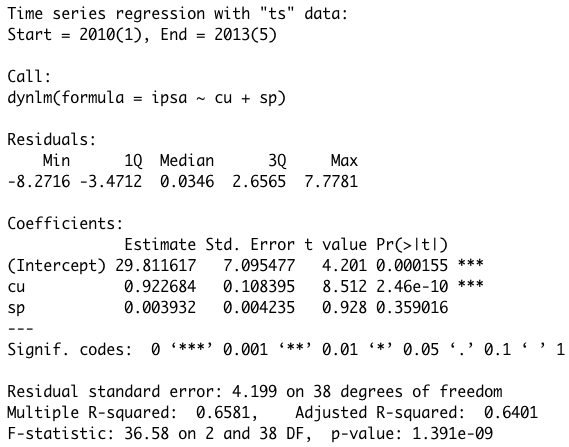
\includegraphics[scale=0.4]{ipsa_cu_sp.png}
\end{figure}

\end{frame}

%---------------------------------------------------------
%---------------------Slide 14--------------------------
\begin{frame}
\frametitle{Cointegration in practice}
\textbf{Ejemplo Modelo IPSA - CU - S$\&$P}

\begin{figure}[t!]
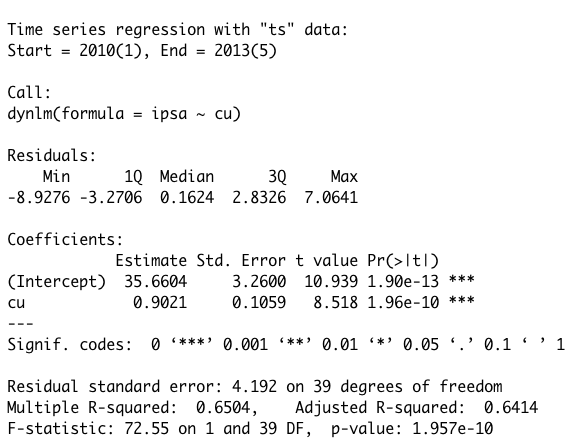
\includegraphics[scale=0.4]{ipsa_cu.png}
\end{figure}
\end{frame}

%---------------------------------------------------------
%---------------------Slide 15--------------------------
\begin{frame}
\frametitle{Cointegration in practice}
\textbf{Ejemplo Modelo IPSA - CU - S$\&$P}

\begin{figure}[t!]
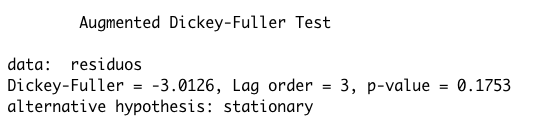
\includegraphics[scale=0.3]{adf_residuos.png}
\end{figure}
\begin{figure}[t!]
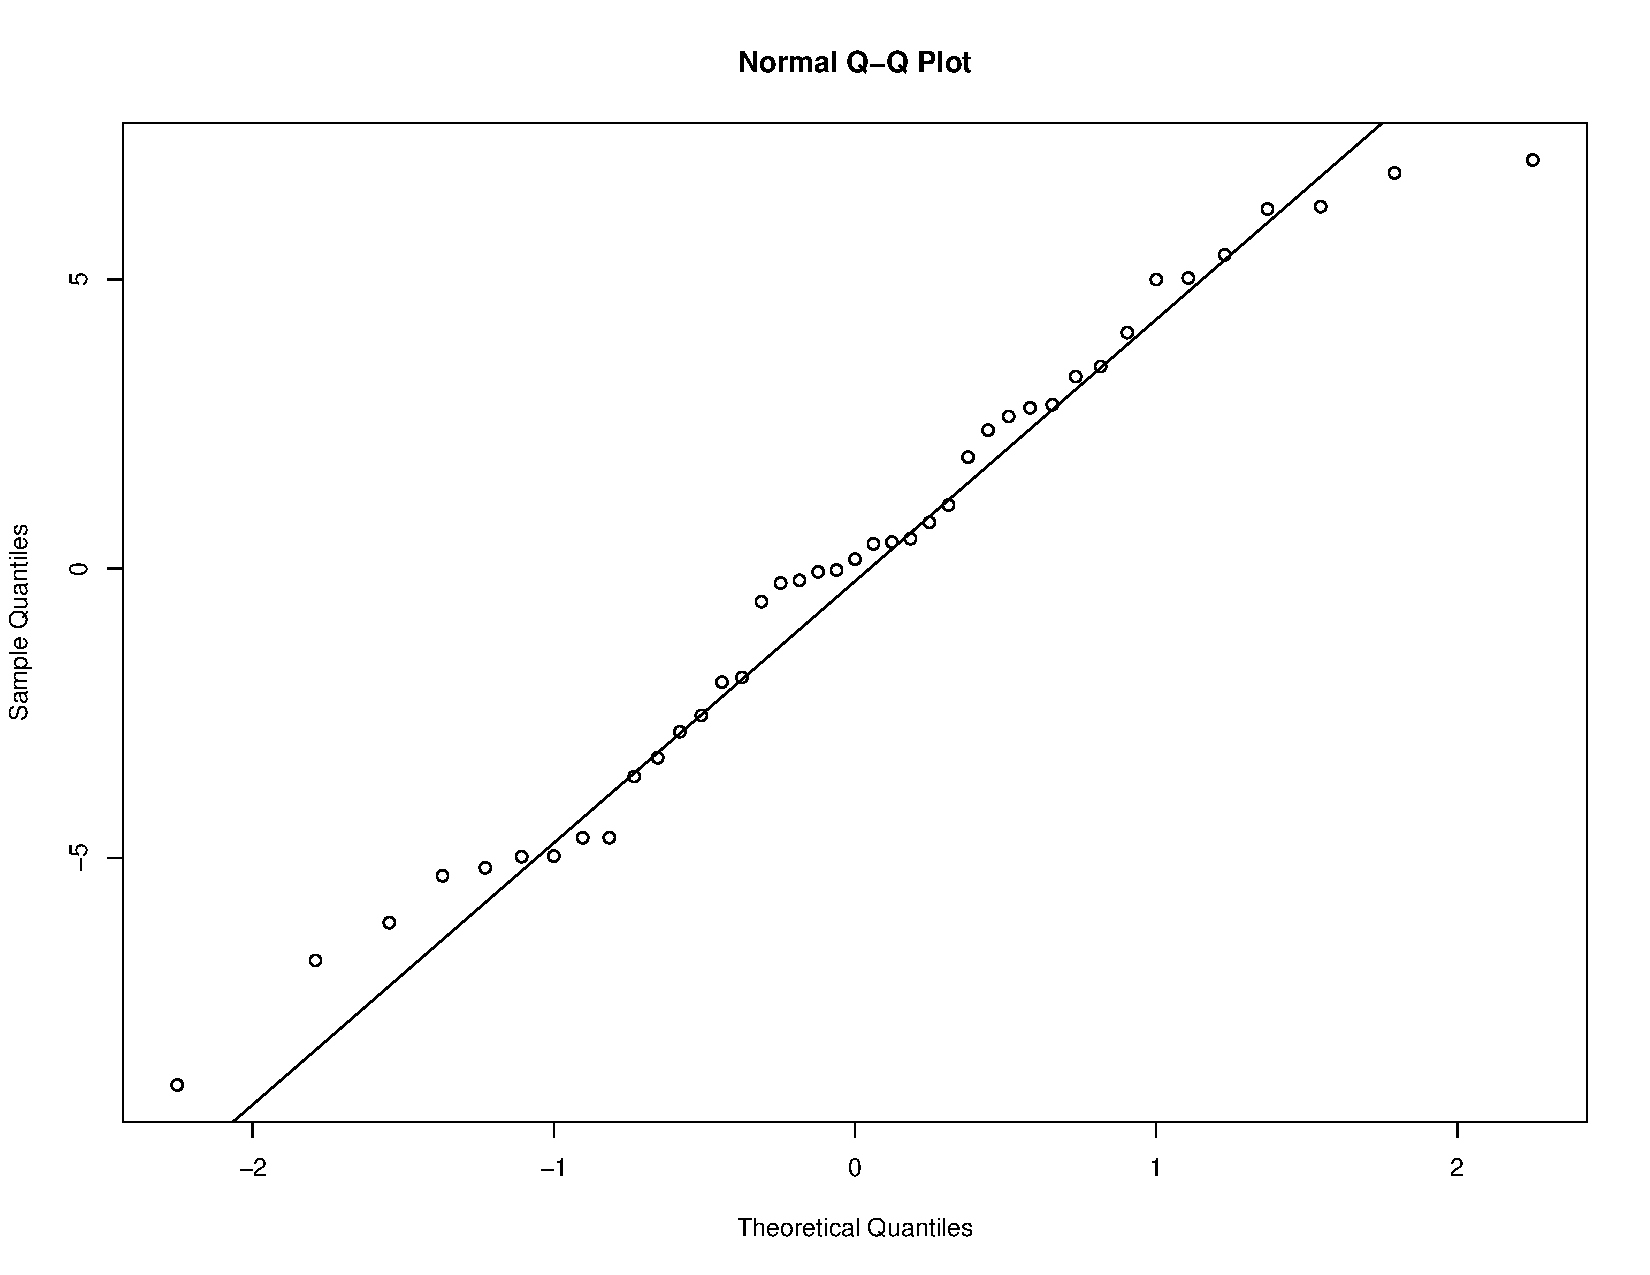
\includegraphics[scale=0.2]{qqres.pdf}
\end{figure}
\end{frame}

%---------------------------------------------------------
%---------------------Slide 16--------------------------
\begin{frame}
\frametitle{Cointegration in practice}
\textbf{Ejemplo Modelo IPSA - CU - S$\&$P}
 \vspace{4mm}	
El ECM usando una regresi\'on din\'amica\\
 \vspace{4mm}	

\only<1|handout:1>{
\begin{exampleblock}{C\'odigo en R}
ipsa.reg4 $<-$ dynlm(diff(ipsa) $\string ~$ diff(cu) + lag(residuos))\\
summary(ipsa.reg4)\\
\end{exampleblock}
}

\end{frame}

%---------------------------------------------------------
%---------------------Slide 17--------------------------
\begin{frame}
\frametitle{Cointegration in practice}
\textbf{Ejemplo Modelo IPSA - CU - S$\&$P}

\begin{figure}[t!]
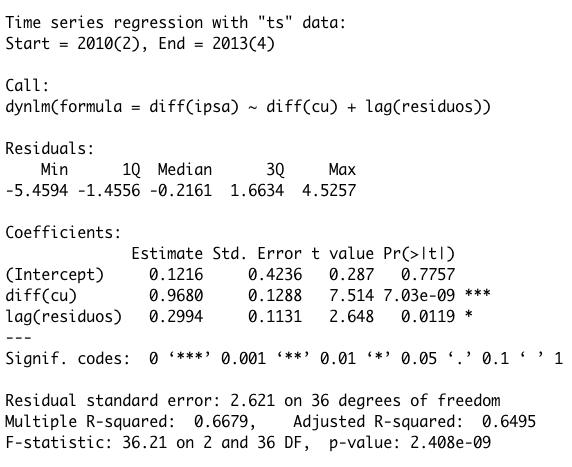
\includegraphics[scale=0.4]{ecm_ipsa_cu.png}
\end{figure}
\end{frame}
\end{section}

%---------------------------------------------------------
%---------------------Slide 18--------------------------

\begin{frame}
\frametitle{Procedimiento de Estimaci\'on}

\textbf{Testing for and Estimating Cointegrating Systems Using the Johansen Technique Based on VARs}\\
\vspace{4mm}	
El test de Johansen, ver \cite{johansen1988statistical},  es una prueba de cointegraci\'on que permite m\'as de una relaci\'on de cointegraci\'on, a diferencia del m\'etodo de Engle-Granger.\\
\vspace{4mm}	
Hay dos tipos de prueba de Johansen, ya sea con traza (trace) o con valor propio (eigenvalue), y las inferencias que pueden ser un poco diferente.\\
\vspace{4mm}	
Esta prueba se basa en la estimaci\'on de m\'axima verosimilitud y dos estad\'{i}sticos: valores propios m\'aximos y una estad\'{i}stica de seguimiento. Esto est\'a relacionado con el rango de la matriz. Si el rango es cero, no hay una relaci\'on de cointegraci\'on. Si el rango es uno, hay uno, si son dos hay dos y as\'{i} sucesivamente.\\
\vspace{4mm}	
En R este procedimiento est\'a automatizado como veremos…

\end{frame}

%---------------------------------------------------------
%---------------------Slide 19--------------------------
\begin{frame}
\frametitle{Cointegration in practice}
\textbf{Ejemplo Modelo IPSA - CU - S$\&$P}

El ECM usando una regresi\'on din\'amica\\
\vspace{4mm}	

\only<1|handout:1>{
\begin{exampleblock}{C\'odigo en R}
install.packages(``urca")\\
library(urca)\\
a$<-$data.frame(ipsa,cu)\\
cointegration $<-$ ca.jo(a, type=``trace", ecdet=``trend", spec=``transitory")\\
summary(cointegration)\\  
\end{exampleblock}
}

\end{frame}

%---------------------------------------------------------
%---------------------Slide 20--------------------------
\begin{frame}
\frametitle{Cointegration in practice}
\textbf{Ejemplo Modelo IPSA - CU - S$\&$P}

\begin{figure}[t!]
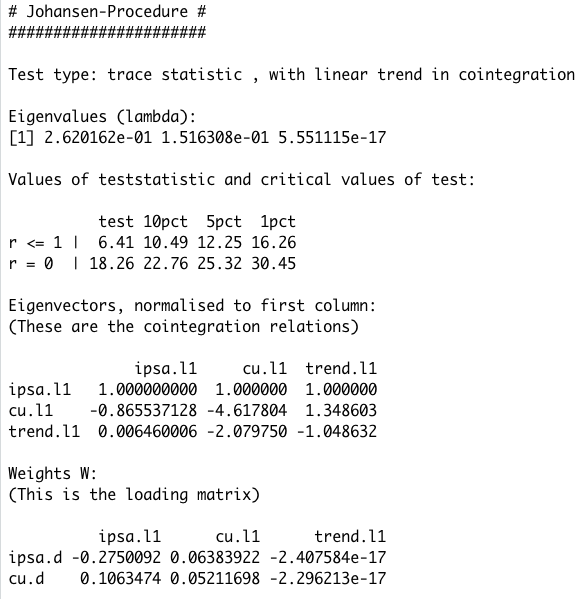
\includegraphics[scale=0.4]{johansen_ipsa_cu.png}

\end{figure}
\end{frame}

%---------------------------------------------------------
%---------------------Slide 21--------------------------
\begin{section}{Cointegration in a VAR: Vector Error-Correction Models}
\begin{frame}
\frametitle{Cointegration in a VAR: Vector Error-Correction Models}


En nuestro an\'alisis VAR, hemos supuesto que las variables del modelo son estacionarias y erg\'odicas. \\
Por otro lado, reci\'en vimos que las variables que son individualmente no estacionarias pueden estar cointegradas. Para el caso simple de dos variables y una relación de cointegraci\'on, vimos que un modelo de correcci\'on de errores es la especificaci\'on econom\'etrica apropiada. \\
\vspace{4mm}	
En este modelo, la ecuaci\'on se diferencia y se incluye un t\'ermino de correcci\'on de errores, que mide la desviaci\'on del per\'{i}odo anterior del equilibrio a largo plazo.\\
Ahora consideramos c\'omo las variables cointegradas se pueden utilizar en un VAR utilizando un modelo vectorial de correcci\'on de errores (\textbf{Vector error correction modelo - VEC model}). 

\end{frame}

%---------------------------------------------------------
%---------------------Slide 22--------------------------
\begin{frame}
\frametitle{Cointegration in a VAR: Vector Error-Correction Models}

\textbf{Un modelo VEC de dos variables}

Si dos series I(1), digamos $Y_t$ y $X_t$, est\'an cointegradas, entonces existe unos \'unicos $\alpha_0$ y $\alpha_1$ tal que $\nu_t = y_t - \alpha_0 - \alpha_1 x_t$ es $I(0)$. En el modelo de cointegraci\'on de una sola ecuaci\'on, vimos que el modelo de correcci\'on de errores:, ten\'{i}a la siguiente forma

\begin{equation}
\triangle y_t = \beta_0 + \beta_1 \triangle x_t + \lambda \nu_{t-1} + \epsilon_t = 
\end{equation}
\begin{equation*}
\beta_0 + \beta_1 \triangle x_t + \lambda (y_{t-1} - \alpha_0 - \alpha_1 x_{t-1} ) + \epsilon_t
\end{equation*}

Todos los t\'erminos en la ecuaci\'on anterior son $I(0)$, siempre que los coeficientes $\alpha$ (el ``vector de cointegraci\'on") sean conocidos o al menos consistentemente estimados. El t\'ermino $\nu_{t -1}$ es la magnitud por la cual $y$ estaba por encima o por debajo de su valor de equilibrio a largo plazo en el per\'{i}odo anterior. El coeficiente $\lambda$ (que esperamos que sea negativo) representa la cantidad de ``correcci\'on" de este per\'{i}odo, (t - 1), desequilibrio que ocurre en el per\'{i}odo t. 

\end{frame}

%---------------------------------------------------------
%---------------------Slide 23--------------------------
\begin{frame}
\frametitle{Cointegration in a VAR: Vector Error-Correction Models}

\textbf{Un modelo VEC de dos variables}

Por ejemplo, si $\lambda$ es - 0.25, entonces un cuarto de la brecha entre $y_{t - 1}$ y su valor de equilibrio tender\'{i}an (todo lo dem\'as igual) a invertirse (porque el signo es negativo) en el período $t$.\\
\vspace{4mm}	
El modelo VEC ampl\'{i}a este modelo de correcci\'on de errores de una sola ecuaci\'on para permitir que $y$ y $x$ evolucionen conjuntamente a lo largo del tiempo como en un sistema VAR. En el caso de dos variables, solo puede haber una relaci\'on de cointegraci\'on y la ecuaci\'on y del sistema VEC es similar a la vista anteriormente, excepto que reflejamos la especificación VAR al poner diferencias desfasadas de $y$ y $x$ en el lado derecho. 

\end{frame}

%---------------------------------------------------------
%---------------------Slide 24--------------------------
\begin{frame}
\frametitle{Cointegration in a VAR: Vector Error-Correction Models}

\textbf{Un modelo VEC de dos variables}
Con solo una diferencia de retraso (puede haber m\'as), se puede escribir un modelo VEC bivariado como:

\begin{equation}
\triangle y_t = \beta_{y0} + \beta_{yy1} \triangle y_{t-1} + \beta_{yx1} \triangle x_{t-1} + \lambda_y (y_{t-1} - \alpha_0 - \alpha_1 x_{t-1} ) + \upsilon^y_t
\end{equation}
\begin{equation}
\triangle x_t = \beta_{x0} + \beta_{xy1} \triangle y_{t-1} + \beta_{xx1} \triangle x_{t-1} + \lambda_x (y_{t-1} - \alpha_0 - \alpha_1 x_{t-1} ) + \upsilon^x_t
\end{equation}

\end{frame}

%---------------------------------------------------------
%---------------------Slide 25--------------------------
\begin{frame}
\frametitle{Cointegration in a VAR: Vector Error-Correction Models}


Nuevamente, los t\'erminos en ambas ecuaciones son $I(0)$ si las variables son
cointegradas con un vector de cointegraci\'on $(1, - \alpha_0, - \alpha_1)$, en otras palabras, si $y_t - \alpha_0 - \alpha_1x_t$ es estacionario.\\
\vspace{4mm}	
Los coeficientes $\lambda$ son nuevamente los coeficientes de correcci\'on de errores, midiendo la respuesta de cada variable al grado de desviaci\'on del equilibrio a largo plazo en el per\'{i}odo anterior. Nosotros esperamos que $\lambda_y < 0$ por la misma raz\'on que antes: si $y_{t -1}$ est\'a por encima de su valor de largo plazo en relaci\'on con $x_{t -1}$ entonces el t\'ermino de correcci\'on de errores entre par\'entesis es positivo y esto deber\'{i}a producir una baja en $y$ en el per\'{i}odo t. 

\end{frame}
\end{section}

%---------------------------------------------------------
%---------------------Slide 26--------------------------
\begin{frame}
\frametitle{Cointegration in a VAR: Vector Error-Correction Models}


El signo esperado de $\lambda_x$ depende del signo de $\alpha_1$. Esperamos que $ \delta \triangle x_t / \delta x_{t-1} = - \lambda_x \alpha_1 < 0$ por la misma raz\'on que esperamos que $\delta \triangle y_t / \delta y_{t-1} = \lambda_y < 0$: si $x_{t-1}$ est\'a por encima de su relaci\'on de largo plazo con $y$, entonces esperamos que $\triangle x_t$ sea negativo, otras cosas constantes.

\end{frame}

%---------------------------------------------------------
%---------------------Slide 27--------------------------
\begin{frame}
\frametitle{Cointegration in a VAR: Vector Error-Correction Models}


Un ejemplo simple y concreto puede ayudar a aclarar el papel de los t\'erminos de correcci\'on de errores en un modelo VEC. Supongamos que la relaci\'on de cointegraci\'on a largo plazo sea $y_t = x_t$, de modo que $\alpha_0 = 0$ y $\alpha_1 = 1$. El t\'ermino de correcci\'on de error entre par\'entesis en cada ecuaci\'on del sistema VAR es ahora $y_{t -1} - x_{t -1}$, la diferencia entre $y$ y $x$ en el per\'{i}odo anterior. \\
Supongamos que debido a schocks previos, $y_{t -1} = x_{t -1} + 1$ o que y está por encima de su relaci\'on de equilibrio a largo plazo con x en una unidad (o,de manera equivalente, $x$ est\'a por debajo de su relaci\'on de equilibrio de largo plazo con $y$ en una unidad). \\


\end{frame}

%---------------------------------------------------------
%---------------------Slide 28--------------------------
\begin{frame}
\frametitle{Cointegration in a VAR: Vector Error-Correction Models}


Para avanzar hacia el equilibrio de largo plazo en el período t, esperamos (si no hay otros cambios) $\triangle y_t < 0$ y $\triangle x_t > 0$. $\triangle y_t$ cambia en respuesta a este equilibrio mediante $\lambda_y (y_{t-1} - x_{t-1}) = \lambda_y$, para que ocurra un ajuste estable, $\lambda_y < 0$; $y$ es demasiada alta, por lo que debe disminuir en respuesta al desequilibrio. El cambio correspondiente en $\lambda_x (y_{t-1} - x_{t-1}) = \lambda_x$. Como x es ``demasiado bajo", el ajuste estable requiere que la respuesta en $x$ sea positiva, por lo que necesitamos $\lambda_x > 0$. Tenga en cuenta que si la relaci\'on a largo plazo entre $y$ y $x$ fuera inversa ($\alpha_1 < 0$), entonces $x$ necesitar\'{i}a disminuir para avanzar hacia el equilibrio y necesitaríamos $\lambda_x < 0$. El signo esperado en $\lambda_x$ depende del signo de $\alpha_1$.

\end{frame}

%---------------------------------------------------------
%---------------------Slide 29--------------------------
\begin{frame}
\frametitle{Cointegration in practice}
\textbf{Ejemplo Modelo IPSA - CU - S$\&$P}

El ECM usando una regresi\'on din\'amica\\
\vspace{4mm}	

\only<1|handout:1>{
\begin{exampleblock}{C\'odigo en R}
library(tsDyn)\\

a$<-$data.frame(ipsa,cu)\\
$\string #$Fit a VECM with Engle-Granger 2OLS estimator:\\
vecm.eg$<-$VECM(a, lag=2)\\
\\
$\string #$Fit a VECM with Johansen MLE estimator:\\
vecm.jo$<-$VECM(a, lag=2, estim=``ML")\\


\end{exampleblock}
}

\end{frame}

%---------------------------------------------------------
%---------------------Slide 30--------------------------
\begin{frame}
\frametitle{Cointegration in a VAR: Vector Error-Correction Models}

\textbf{Un modelo VEC de dos variables}

\begin{figure}[t!]
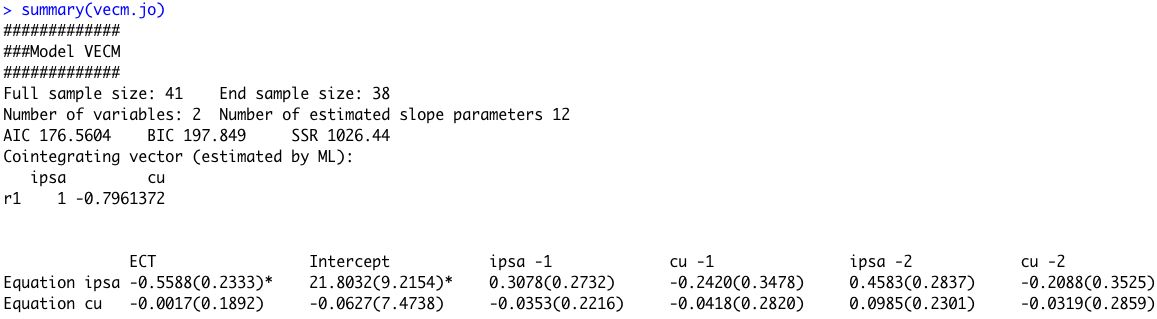
\includegraphics[scale=0.35]{vecm_ipsa_cu_ML.png}
\end{figure}
\begin{figure}[t!]
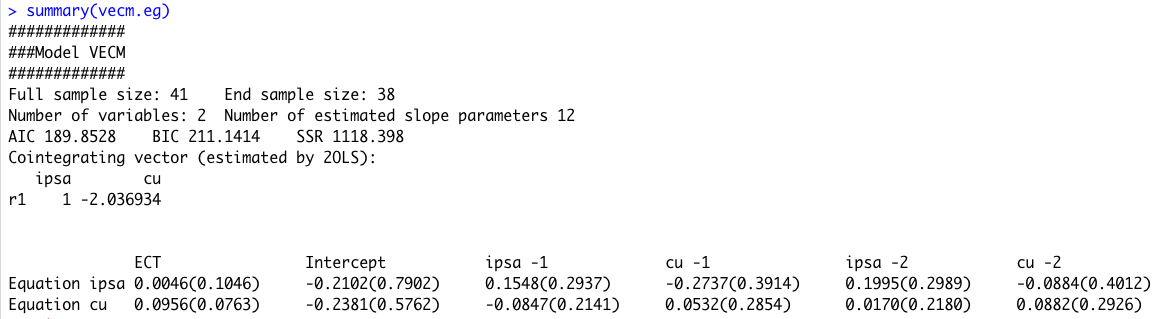
\includegraphics[scale=0.35]{vecm_ipsa_cu_2OLS.png}
\end{figure}

\end{frame}
\end{section}


%---------------------------------------------------------

%---------------------Slide 31--------------------------
\begin{section}{Cointegration con Modelos ARDL}
\begin{frame}
\frametitle{Cointegration con Modelos ARDL}

La t\'ecnica de cointegraci\'on ARDL, ver \cite{pesaran2001bounds}, no requiere pruebas previas para ra\'{i}ces unitarias a diferencia de otras m\'etodos. En consecuencia, la t\'ecnica de cointegración ARDL es preferible cuando
lidiamos con variables que est\'an integradas con diferente orden, $I(0)$, $I(1)$ o una combinaci\'on de las dos.\\
La relaci\'on a largo plazo de las variables subyacentes se detecta a trav\'es del estad\'{i}stico F (prueba de Wald). En este enfoque, la relaci\'on a largo plazo de la serie se establece cuando el Fstatistic excede la banda de valor cr\'{i}tico. La gran ventaja de este enfoque radica en su identificaci\'on de los vectores de cointegraci\'on donde hay m\'ultiples vectores cointegrantes.

\end{frame}

%---------------------------------------------------------
%---------------------Slide 32--------------------------
\begin{frame}
\frametitle{Cointegration in practice}
\textbf{Ejemplo Modelo IPSA - CU - S$\&$P}

\only<1|handout:1>{
\begin{exampleblock}{C\'odigo en R}

ipsa.reg4 $<-$ auto.ardl(ipsa $\string ~$ cu)\\
ipsa.reg4 $<-$ ardl(ipsa $\string ~$ cu)\\

\end{exampleblock}
}

\end{frame}

\end{section}

%---------------------------------------------------------
%--------------Slide Referencias---------------------

\section{Referencias}
\begin{frame}[allowframebreaks]
        \frametitle{Referencias}
        \bibliographystyle{unsrt}
        \nocite{} %lista sin citar.
        \bibliography{TS_ref}
\end{frame}
\end{section}

%---------------------------------------------------------
%---------------------------------------------------------
\end{document} 
%---------------------------------------------------------




